\PassOptionsToPackage{dvipsnames,table}{xcolor}
\documentclass[11pt,a4paper]{article}

\usepackage{DS}

\begin{document}

\input{\detokenize{/home/fenarius/Travail/Cours/cpge-info/latex/Macros.tex}}
\ModeConcours
\DS{MP2I}{7}{Juin 2025}

\setboolean{corrige}{false}
\newcommand{\non}{\neg}
\newcommand{\et}{\wedge}
\newcommand{\ou}{\vee}
\newcommand{\imp}{\to}
\newcommand{\eq}{\leftrightarrow}


\newcommand{\maillon}[3]{
	\begin{tabular}{|p{0.2cm}|p{0.2cm}|}
		\hline
		\rnode{#2}{#1} & \rnode{#3}{\phantom{$e_0$}} \\
		\hline
	\end{tabular}
}

\alertbox{\danger}{Consignes}{
	\begin{itemize}
		\item[\textbullet] Les programmes demandés doivent être écrits en C ou en OCaml suivant l'exercice. Dans le cas du C, on suppose que les librairies standards usuelles ({\tt <stdio.h>}, {\tt <stdlib.h>}, {\tt <stdbool.h>}) sont déjà importées.
		\item[\textbullet] On pourra toujours librement utiliser une fonction demandée à une question précédente même si cette question n'a pas été traitée.
		\item[\textbullet] Veillez à présenter vos idées et vos réponses partielles même si vous ne trouvez pas la solution complète à une question.
		\item[\textbullet] La clarté et la lisibilité de la rédaction et des programmes sont des éléments de notation.
	\end{itemize}
}


\begin{Exercise}[title = {L'accès aux enfers}]\\
	Dans la mythologie grecque, l’accès aux Enfers est gardé par le Cerbère, un terrible loup à trois têtes. Celui-ci se trouve devant trois couloirs qui, soit
	permettent de rejoindre le monde des vivants, soit conduisent directement aux Enfers.

	Lorsque Cerbère accueille un nouvel arrivant, il est contraint de lui dire la vérité. Par la suite, il peut mentir ou dire la vérité à sa guise mais il respecte toujours les règles qu’il s’est fixées.

	Après avoir bu la coupe de ciguë, Socrate se retrouve face à Cerbère. Celui-ci, honoré de rencontrer le grand philosophe, veut lui offrir une chance d’éviter la damnation éternelle. Il lui dit alors : \og{} \textit{Je vais t’indiquer un des couloirs qui mène au monde des vivants mais, pour mettre à l’épreuve ta grande sagesse, j’énoncerai trois indications logiques qui seront, soit toutes vraies, soit toutes fausses et tu en déduiras le couloir que tu devras suivre} \fg{}.

	Nous noterons $I_1$ , $I_2$ et $I_3$ les propositions associées aux indications de la première, la deuxième et la troisième tête de Cerbère.
	\Question{Représenter l'énoncé de Cerbère sous la forme d'une formule du calcul des propositions dépendant de $I_1, I_2$ et $I_3$}
	\tcor{$(I_1 \et I_2 \et I_3) \ou (\non I_1 \et \non I_2 \et \non I_3)$}

	\NRet \smallskip
	La première tête dit ensuite : \og{} \textit{Le premier couloir ainsi que le troisième mènent au monde des vivants} \fg{}.
	La deuxième tête dit : \og{} \textit{Si le deuxième couloir mène au monde des vivants, alors le troisième n'y mène pas \fg{}.}
	La troisième tête conclut par : \og{} \textit{Le premier couloir mène au monde des vivants, par contre le deuxième n'y mène pas \fg{}.}

	Nous noterons, $C_1, C_2$ et $C_3$ les variables propositionnelles correspondant au fait que le premier, le deuxième et le troisième couloir mène au monde des vivants.

	\Ret \smallskip
	\Question{Exprimer $I_1, I_2$ et $I_3$ sous la forme du calcul des propositions dépendant de $C_1, C_2$ et $C_3$}
	\tcor{\begin{itemize}
			\item $I_1 : C_1 \et C_3$
			\item $I_2 : C_2 \imp \non C_3$
			\item $I_3 : C_1 \et \non C_2$
		\end{itemize}}
	\Question{En utilisant le calcul des propositions (résolution avec les tables de vérité), déterminer le couloir que Socrate doit suivre pour rejoindre le monde des vivants.}
	\tcor{
		\begin{tabular}{|l|l|l|l|l|l|l|}
			\hline
			$C_1$ & $C_2$ & $C_3$ & $I_1$ & $I_2$ & $I_3$ & $(I_1 \et I_2 \et I_3) \ou (\non I_1 \et \non I_2 \et \non I_3)$ \\
			\hline
			0     & 0     & 0     & 0     & 1     & 0     & 0                                                                \\
			\hline
			0     & 0     & 1     & 0     & 1     & 0     & 0                                                                \\
			\hline
			0     & 1     & 0     & 0     & 1     & 0     & 0                                                                \\
			\hline
			0     & 1     & 1     & 0     & 0     & 0     & 1                                                                \\
			\hline
			1     & 0     & 0     & 0     & 1     & 1     & 0                                                                \\
			\hline
			1     & 0     & 1     & 1     & 1     & 1     & 1                                                                \\
			\hline
			1     & 1     & 0     & 0     & 1     & 0     & 0                                                                \\
			\hline
			1     & 1     & 1     & 1     & 0     & 0     & 0                                                                \\
			\hline
		\end{tabular}\\
		Donc comme $I_1, I_2$ et $I_3$ sont soient toutes vraies soient toutes fausses, seules deux lignes du tableau conviennent et dans les deux cas, $C_3$ est vraie, donc pour être sur de rejoindre le monde des vivants, Socrate doit prendre le couloir 3.
	}
	\Question{En admettant que Cerbère ait menti en donnant les trois indications, Socrate pouvait-il suivre d'autres couloirs ? Si oui, le ou lesquels ?}
	\tcor{Si on suppose que Cerbère a menti alors on se trouve sur la ligne où $I_1, I_2$ et $I_3$ sont fausses et donc deux couloirs permettent de rejoindre le monde des vivants le couloir 2 et le couloir 3.}
\end{Exercise}

\begin{Exercise}[title = Séquence génétique]\\
	On s'intéresse dans cet exercice à la compression de chaines de caractères représentant des séquences génétiques codées sur l'alphabet {\tt \{A, C, G, T\}}. Et on souhaite compresser la séquence $S$={\tt ATGTGATGTCCT}. On supposera qu'initialement la séquence est codée en {\sc ascii} et que donc chacun des caractères occupe 1 octet (donc 8 bits).
	\Question{Construire l'arbre de Huffman associé à la compression de $S$.}
	\tcor{
		\begin{center}
			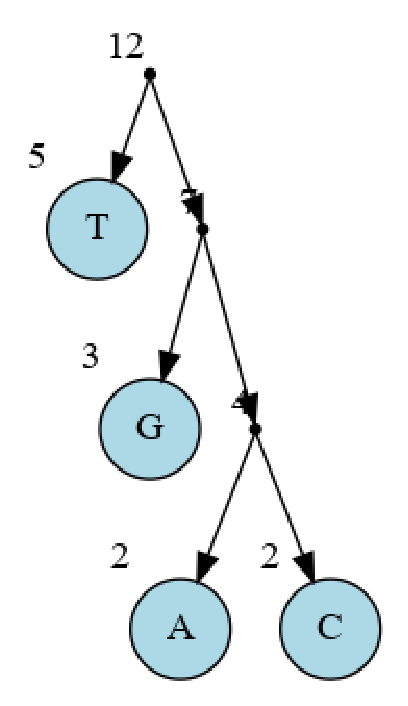
\includegraphics[height=5cm]{hf.eps}
		\end{center}
	}
	\Question{Donner les codes obtenus pour chacun des quatre caractères {\tt A, C, G} et {\tt T}. En déduire le taux de compression de l'algorithme, sans tenir compte de la taille de l'arbre (on pourra conserver une écriture fractionnaire).}
	\tcor{
	\begin{itemize}
		\item Code pour {\tt T} = {\tt 0}
		\item Code pour {\tt G} = {\tt 10}
		\item Code pour {\tt A} = {\tt 110}
		\item Code pour {\tt C} = {\tt 111}
	\end{itemize}

	\Ret
	Comme indiqué sur l'arbre {\tt T} apparaît 5 fois, {\tt G} 3 fois et {\tt A} et {\tt C} chacun deux fois. La taille finale du code est donc : $5 \times 1 + 3\times 2 + 2\times 3 + 2 \times 3 = 23$ bits, alors le code initial contenait $12$ caractères codés sur 8 bits chacun donc $96$ octets, le taux de compression est donc de $\dfrac{23}{96} \simeq 24 \%$.
	}

	\NRet \smallskip
	On rappelle que le principe de la compression {\sc lzw} est d'attribuer un code aux préfixes rencontrés lors de la lecture du texte à compresser de façon à disposer d'un code compact si ce préfixe se présente à nouveau.  On attribue initialement les codes {\tt A} $\rightarrow 0$, {\tt C} $\rightarrow 1$, {\tt G} $\rightarrow 2$  et {\tt T} $\rightarrow 3$
	Le début de l'algorithme va donc consister à attribuer un nouveau code au premier préfixe non encore codé qui apparaît lors de la lecture du texte. Et donc, ici, on attribue le code {\tt 4} au prefixe {\tt AT} et on émettra le code de {\tt A} c'est à dire 0.

	\Ret\smallskip
	\Question{Poursuivre le déroulement de cet algorithme en complétant le tableau suivant : \\
		\begin{tabular}{|l|l|l|}
			\hline
			Position dans le texte          & Code émis & Nouveau préfixe ajouté    \\
			\hline
			{\tt \underline{A}TGTGATGTCCT } & 0         & {\tt AT } $\rightarrow 4$ \\
		\end{tabular}\\
	}
	\tcor{
	\begin{tabular}{|l|l|l|}
		\hline
		Position dans le texte         & Code émis & Nouveau préfixe ajouté     \\
		\hline
		{\tt \underline{A}TGTGATGTCCT} & 0         & {\tt AT } $\rightarrow 4$  \\
		\hline
		{\tt A\underline{T}GTGATGTCCT} & 3         & {\tt TG } $\rightarrow 5$  \\
		\hline
		{\tt AT\underline{G}TGATGTCCT} & 2         & {\tt GT } $\rightarrow 6$  \\
		\hline
		{\tt ATG\underline{TG}ATGTCCT} & 5         & {\tt TGA } $\rightarrow 7$ \\
		\hline
		{\tt ATGTG\underline{AT}GTCCT} & 4         & {\tt ATT } $\rightarrow 8$ \\
		\hline
		{\tt ATGTGAT\underline{GT}CCT} & 6         & {\tt GTT } $\rightarrow 9$ \\
		\hline
		{\tt ATGTGATGT\underline{C}CT} & 1         & {\tt CC } $\rightarrow 10$ \\
		\hline
		{\tt ATGTGATGTC\underline{C}T} & 1         & {\tt CT } $\rightarrow 11$ \\
		\hline
		{\tt ATGTGATGTCC\underline{T}} & 3         &                            \\
		\hline
	\end{tabular}\\
	On obtient donc la suite de codes : {\tt [0; 3; 2; 5; 4; 6; 1; 1; 3]}}
	\Question{Quel est le taux de compression obtenu (la taille d'un code est un octet) ?}
	\tcor{12 sur 9}
	\Question{Décompresser le texte $T$ codé par suite de codes {\tt [3; 1; 4; 6; 5; 2; 0; 2 ]} sur ce même alphabet en expliquant comment est reconstruit le dictionnaire de décompression.}
	\tcor{$T = $ {\tt TCTCTCTCTGAG}}
\end{Exercise}



\begin{Exercise}[title = {Triangle dans un graphe}]\\
	On considère un graphe \textit{non orienté} $G = (S,A)$ où $A = \{0, \dots, n-1 \}$. On dit qu'un sous ensemble de $V$ à trois éléments $\{x,y,z\}$  est un \textit{triangle} de $G$ lorsque $\{x,y\}, \{y, z\}$ et $\{x, z\}$ appartiennent à $A$.
	Par exemple, dans le graphe  suivant, $\{0, 1, 3\}$ est un triangle car $\{0, 1\}, \{1, 3\}$ et $\{0,3\}$ sont des arcs mais $\{0, 1, 2\}$ n'est pas un triangle car $\{0, 2\}$ n'est pas un arc.
	\begin{center}
		\begin{pspicture}(0,-2.2)(5,1)
			\rput(1,0){\circlenode{x1}{$0$}}
			\rput(3,0){\circlenode{x2}{$1$}}
			\rput(5,-1){\circlenode{x3}{$2$}}
			\rput(1,-2){\circlenode{x4}{$3$}}
			\rput(3,-2){\circlenode{x5}{$4$}}
			\ncline{-}{x1}{x2}
			\ncline{-}{x1}{x4}
			\ncline{-}{x1}{x5}
			\ncline{-}{x2}{x1}
			\ncline{-}{x2}{x5}
			\ncline{-}{x2}{x4}
			\ncline{-}{x2}{x3}
			\ncline{-}{x3}{x2}
			\ncline{-}{x3}{x5}
			\ncline{-}{x4}{x5}
		\end{pspicture}
	\end{center}
	\Question{Donner tous les triangles du graphe $g$.}
	\tcor{On obtient : {\tt \{ 0, 1, 3\}, \{ 0, 1, 4\}, \{ 0, 3, 4\}, \{ 1, 2, 4\} et \{ 1, 3, 4\}}}
	\Question{Rappeler la définition d'un graphe complet. Donner le nombre de triangle d'un graphe complet à $n$ sommets.}
	\tcor{Un graphe complet est un graphe dans lequel pour toute paire de sommets $(i,j)$, on a $ij$ qui est un arc c'est à dire $ij \in A$. Donc tous les triplets de sommets sont des triangles, donc il y a autant de triplets de sommets que de triangle, c'est à dire $\displaystyle{\binom{|S|}{3}}$ triangles}
	\Question{On rappelle qu'un graphe est \textit{bipartite} lorsqu'il existe une partition de l'ensemble des sommets $S$ en deux ensembles $S_1$ et $S_2$ tel que tout arête ait un élément dans $S_1$ et l'autre dans $S_2$. Montrer qu'un graphe bipartite ne contient pas de triangles.}
	\tcor{Soit $ij \in A$, et quitte à échanger leurs rôles supposons $i \in S_1$ et $j \in S_2$, alors pour tout autre sommet $k$ du graphe, soit $k \in S_1$ et donc $ik \notin A$ , soit $k \in S_2$ et donc $kj \notin A$. Donc $ijk$ n'est pas un triangle.}
	\Question{Afin de lister les triangles d'un graphe, on propose de tester si chaque partie de $S$ à 3 éléments est un triangle. Donner la complexité d'un tel algorithme en fonction du nombre de sommets $|S|$ du graphe.}
	\tcor{Il faut tester les $\displaystyle{\binom{|S|}{3} = \dfrac{|S|(|S|-1)(|S|-2)}{6}}$ parties possibles à 3 éléments, cet algorithme a donc une complexité quadratique $\mathcal{O}(|S|^3)$ en nombre de sommets du graphe.}
	\Question{Un autre algorithme possible pour lister les triangles d'un graphe consiste pour chaque arête $\{x,y\}$ à chercher l'ensemble des sommets $z$ adjacent à $x$ et à $y$. Ce qui revient à déterminer l'intersection des listes d'adjacences de $x$ et de $y$. Donner la complexité de cet algorithme (en fonction de $|A|$ et de $|S|$) si on suppose que l'intersection de deux listes est calculée en temps linéaire du minimum de leur nombre de sommet, c'est à dire que la complexité du calcul de l'intersection de {\tt l1} (longueur {\tt n1}) et {\tt l2} (longueur {\tt n2} est un $\mathcal{O}(\min(n1, n2))$). \label{ai}}
	\tcor{Cette fois, on parcourt l'ensemble des arêtes, et  pour chaque arête, on doit calculer l'intersection de deux listes contenant au plus $|S|$ éléments et ce calcul est supposé se faire en $\mathcal{O}(|S|)$, donc on obtient une complexité en $\mathcal{O}(|S||A|)$.}
	\Question{Ecrire en OCaml, une fonction {\tt intersection int list -> int list -> int list} qui calcule en temps linéaire l'intersection de deux listes \textit{en les supposant triées}.}
	\ifcorrige
		\corpartOCaml{triangle_graphe.ml}{}{}{10}{16}
	\fi
	\Question{Dans la suite de l'exercice, on utilise des graphes représentés par liste d'adjacence en OCaml avec le type :
		\inputpartOCaml{triangle_graphe.ml}{}{}{2}{4}
		Ecrire une fonction {\tt ajoute graphe -> int -> int -> ()} permettant d'ajouter une arête dans un graphe en \textit{maintenant triées} les listes d'adjacence. On pourra supposer qu'on ajoute toujours un arc qui n'existe pas encore dans le graphe.
	}
	\ifcorrige
		\corpartOCaml{triangle_graphe.ml}{}{}{18}{24}
	\fi
	\Question{Implémenter l'algorithme décrit à la question \textbf{Q14-} pour lister les triangles d'un graphe en écrivant une fonction {\tt triangle : graphe -> (int*int*int) list} qui renvoie la liste des triangles du graphe.}
\end{Exercise}

\end{document}